\documentclass[9pt,twocolumn,twoside,lineno]{pnas-new}
% Use the lineno option to display guide line numbers if required.

% packages
\usepackage{courier}

\templatetype{pnasresearcharticle} % Choose template 
% {pnasresearcharticle} = Template for a two-column research article
% {pnasmathematics} %= Template for a one-column mathematics article
% {pnasinvited} %= Template for a PNAS invited submission

\title{Genomic architecture controls multivariate adaptation to climate change}

% Use letters for affiliations, numbers to show equal authorship (if applicable) and to indicate the corresponding author
\author[a,1]{Drew E. Terasaki Hart}
\author[a]{Ian J. Wang}

\affil[a]{Department of Environmental Science, Policy, and Management, University of California, Berkeley, CA 94720}

% Please give the surname of the lead author for the running footer
\leadauthor{Terasaki Hart} 

% Please include corresponding author, author contribution and author declaration information
\authorcontributions{D.E.T.H. conceived, designed and wrote the simulations and analysis, and wrote the manuscript. I.J.W. helped conceive and design the simulations and analysis, and cowrote the manuscript.}
\authordeclaration{The authors declare no competing interests.}
\correspondingauthor{\textsuperscript{1}To whom correspondence should be addressed. E-mail: drew.hart@berkeley.edu}

% At least three keywords are required at submission. Please provide three to five keywords, separated by the pipe symbol.
\keywords{adaptation $|$ climate change $|$ $|$ landscape genomics $|$ spatial simulation $|$ gene flow $|$ genetic architecture} 

\begin{abstract}
Please provide an abstract of no more than 250 words in a single paragraph. Abstracts should explain to the general reader the major contributions of the article. References in the abstract must be cited in full within the abstract itself and cited in the text.

Multivariate selective environments have
profound potential evolutionary importance,
yet have been largely ignored in most
research on climate change adaptation.

Our analysis provides important theoretical insights
into the nature of polygenic adaptation under multivariate environmental change,
a neglected area of research.
While we confirm that some principles derived from previous models of local adaptation to static environments
also apply to changing environments, we simultaneously
reveal dynamics that would not be evident on that basis.
Our results generally support the first-order assumption underlying AGF,
but also suggest that if theoretical landscape genetics can cast 
light on the processes underlying maladaptation, adaptive capacity, and adaptive gene
flow, it can help answer the fundamental question posed by AGF: Whom to move where?

\end{abstract}

% Please add a significance statement to explain the relevance of your work
\significancestatement{Authors must submit a 120-word maximum statement about the significance of their research paper written at a level understandable to an undergraduate educated scientist outside their field of speciality. The primary goal of the significance statement is to explain the relevance of the work in broad context to a broad readership. The significance statement appears in the paper itself and is required for all research papers.}

\dates{This manuscript was compiled on \today}
\doi{\url{www.pnas.org/cgi/doi/10.1073/pnas.XXXXXXXXXX}}

\begin{document}

\maketitle
\thispagestyle{firststyle}
\ifthenelse{\boolean{shortarticle}}{\ifthenelse{\boolean{singlecolumn}}{\abscontentformatted}{\abscontent}}{}


%%%%%%%%%%%%%%%%%%%%%%%%%%%%%%%%%%%%%%%%%%%%%%%%%%%%%
%TODO:
%0. I bet the apparent inversion of gene flow results could have something to do with how I swapped the linkage and genicity orderds before running final batches of high-redundancy sims!! Look into this to confirm, but then I just need to figure out how to run the high-redund scenarios to completion without swapping the order (perhaps just hacky: add `if linkage != 'high': <SKIP>` statement?)
%1. finalize redundancy plots (change teal and red to some other colors not close to those used elsewhere in the study?)
%2. run final set of sims after 05/31, then add final figures here
%3. write any final stats tests? (pheno-shift ANOVA using redund and non-redund combined? test for directions?)
%4. do once-over of methods and finalize
%6. panel together population density plots for all scenarios, identically to panelled maladaptation plots
%7. add and reference maladaptation plots for high-redundancy non-null sims and for null sims
%%%%%%%%%%%%%%%%%%%%%%%%%%%%%%%%%%%%%%%%%%%%%%%%%%%%%


\dropcap{C}limate change is one of the foremost threats to biodiversity in the Anthropocene.
Species’ persistence within their current ranges is likely to depend largely upon their ability to
adapt to climate change through natural selection - a concept frequently referred to 
as `adaptive capacity’ (or `evolutionary potential’;
\cite{chevin,harrisson,nicotra,vilas,wade}).
Given the long expected wait times to adaptive \textit{de novo} mutations,
it is generally assumed that this adaptation will be facilitated
by reconfiguration of a species' existing adaptive diversity.
One conceptual model underlying this assumption is that of
adaptive gene flow parallel to a shifting climatic gradient
(i.e., in the vector
direction of climate velocity; \cite{ackerly}),
which would bring pre-adapted genes into recipient populations
from 'climate-suitable' populations
whose current climates approximate future local projections \cite{bellis}.
This model of adaptive gene flow has both theoretical
\cite{aitken_whitlock,slatkin,tigano}
and empirical 
\cite{feder,bell}
support,
but meets resistance in theoretical conditions under which gene flow can be maladaptive
\cite{wang,lenormand,slatkin,haldane,wright,felsenstein}.
In these circumstances, shifting allelic covariance --- 
i.e., \textit{in situ} recombination of standing genetic variation into new,
adaptive genotypes --- could be a more efficient mechanism of local adaptation to change.

In recent decades, research bridging the fields
of molecular population genetics
and quantitative genetics
\cite{barghi_polygenic,barton,pritchard_human_adaptation,pritchard_sweeps_alone}
has revealed that the genetic architecture of a trait
is a core determinant of whether and how that trait
becomes locally adapted \cite{yeaman_review}.
The number of loci underlying a trait (henceforth, 'polygenicity'),
the rate of recombination between trait loci (i.e., linkage),
and the number of distinct genotypes that yield identical trait phenotypes
(i.e., genetic redundancy; \cite{yeaman_review,laruson,barghi_polygenic})
are among the key influential aspects of genetic architecture
\cite{barton,yeaman_whitlock,yeaman_review,lecorre}.
Polygenicity affects the efficiency of natural selection,
and previous research suggests ecologically-relveant traits can vary from
few loci of large effect
\cite{martin,rees}
to many loci of small but non-negligible effect
\cite{boyle,rockman,savolainen,sella,barghi_polygenic}.
Linkage controls the likelihood that adaptive alleles cluster together,
essentially forming larger-effect-size alleles that are more 
effective targets of selection and are more resistant
to swamping gene flow \cite{yeaman_whitlock}
and facilitating local adaptation \cite{tigano}.
Genetic redundancy can facilitate local adaptation 
by allowing a stable phenotypic cline to exist as a dynamic equilibrium
of continuous and concerted shifts in allele frequencies
(i.e., 'transient genetic architectures' \cite{barghi_redundancy,manceau,yeaman_amnat}).

The influence of genetic architecture on the nature and outcomes
of local adaptation to changing environmental gradients
has been studied to a limited extent,
with nearly exclusive focus on univariate models
of the selective environment (but see \cite{schiffers}).
Such models are inadequate for studying adaptation to climate change
because species are often simultaneously adapted to multiple, unaligned environmental gradients
(be they climatic, physiographic, edaphic, or biotic),
and these gradients may shift differentially and thus decouple as climate changes
\cite{crimmins,daly},
leading to the emergence of novel multivariate landscapes
\cite{williams_novel_climates,williams_projected_novel_disappearing,fitzpatrick_climate_novelty_forecasts}.
Under these circumstances,
even gene flow from 'climate-suitable' populations
could be maladaptive when viewed holistically, if
incoming haplotypes have conflicting fitness effects
on each of the traits adapted to the decoupling gradients,
such that the evolutionary outcome could depend on
the genetic architecture of the traits involved
\cite{aitken_whitlock,schiffers}.
The relative magnitudes of the maladaptive nature of gene flow
and the maladaptation present within a recipient population,
which depend on the polygenicity, redundancy, and linkage of the traits involved,
may determine the relative contributions of gene flow
and of \textit{in situ} shifts in allelic covariance
to the process of adaptation to climate change --- and indeed,
whether a species adapts to climate change at all.

Spatially explicit simulation is one of the strongest available tools
for improving our understanding of maladaptation and adaptive capacity
under climate change \cite{capblancq_review}.
In this study, we use individual-based, spatially explicit simulations
to test how genetic architecture influences multivariate adaptation to climate change.
We first simulate 
adaptation of a population to a bivariate environment composed of two horizontal 
environmental gradients, each exerting selection on a separate trait.
In our main models, we then simulate climate change on that landscape by holding one gradient 
constant while gradually shifting the other gradient horizontally, such that
the decoupling environment pushes the local fitness peaks toward novel regions 
of bivariate trait space (Fig. \ref{fig:conceptual}).
We run 100 pairs of main (changing-climate)
and null (stable-climate) simulations, for each of eighteen scenarios
resulting from the full factorial crossing of:
\begin{enumerate}
    \item two levels of \textbf{redundancy} (low: genotype-phenotype mapping is many-to-one for mid-range phenotypes, but reduces to one-to-one at extreme phenotypes; high: all phenotypes have many-to-one genotype-phenotype mappings; see Fig. S3); 
    \item three levels of \textbf{polygenicity} (low: 4 loci per trait for low-redundancy scenarios, 8 loci per trait for high; moderate: 20 and 40 loci per trait; and high: 100 and 200 loci per trait);
    \item three levels of \textbf{linkage} between all loci (independent: recombination rate ($r$) = 0.5; weak linkage: $r$ = 0.05; and strong linkage: $r$ = 0.005).
\end{enumerate}


\begin{figure}%[tbhp]
\centering
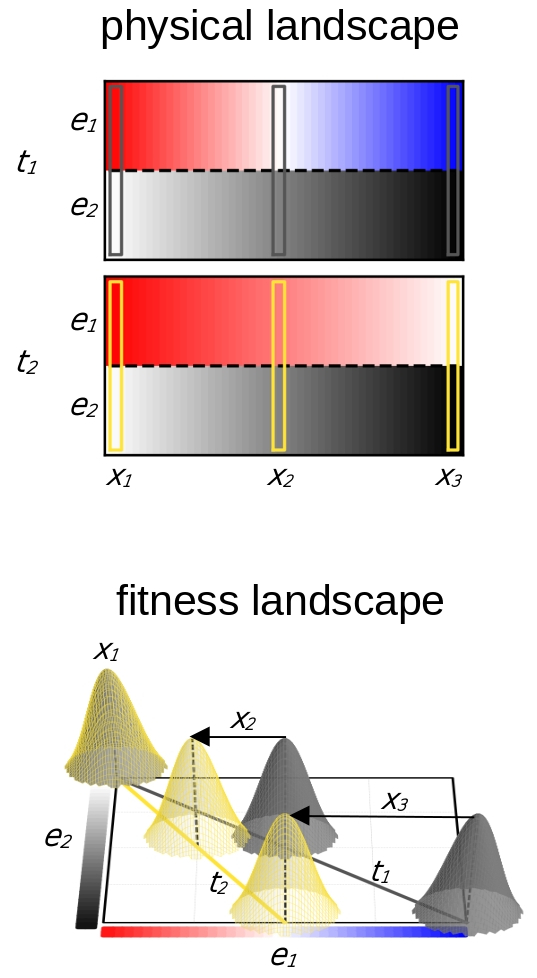
\includegraphics[width=.8\linewidth]{conceptual_fig/ch2_conceptual_fig_crop}
    \caption{Conceptual model of adaptation climate change. Above: Stacked, horizontal cross-sections of our square simulation landscape, shown for the shifting environmental gradient ($e_{1}$, blue-red color ramp) and the stable gradient ($e_{2}$, white-black color ramp), both before climate change ($t_{1}$) and after ($t_{2}$). Below: Bivariate fitness landscape of the traits adapted to the shifting and stable gradients, on axes $e_{1}$ and $e_{2}$, respectively. Three example positions along the bivariate gradient ($x_{1}$, $x_{2}$, $x_{3}$) are delineated by thin vertical boxes on the physical landscape, both before climate change (gray) and after (yellow), and their corresponding fitness peaks are shown as color-matched kernels located along color-matched lines of the fitness optima that exist on the physical landscape before ($t_{1}$) and after ($t_{2}$) climate change. Shifts in local fitness peaks are shown as labeled arrows ($x_{2}$, $x_{3}$); the environment at the far left of the physical landscape does not change, so $x_{1}$'s fitness peaks are overlapping and have no shift, whereas the environment at the far right of the physical landscape experiences the maximal rate of change, which is reflected in the shift in $x_{3}$'s fitness peaks. Note that fitness peaks are stylized and truncated for ease of depiction; fitness in our models decreases linearly with an individual's distance from its phenotypic optimum, rather than the truncated Gaussian functiondepicted here.}
\label{fig:conceptual}
\end{figure}


We test the hypotheses that:
\begin{enumerate}
    \item Up-gradient gene flow is higher under climate change than in null scenarios, having at least some adaptive value, but contributes least to adaptation in lower-linkage, high-polygenicity scenarios, where \textit{in situ} restructuring of allelic covariance among many small-effect alleles, akin to adaptation under transient genetic architectures, can drive phenotypic shifts that are not maladaptive with respect to the stable gradient.
    \item Stronger linkage and higher polygenicity reduce adaptive capacity under sudden climate change (i.e.,  result in greater reductions in population size and in mean fitness, and more persistent maladaptation), because both conditions require longer expected wait times for the emergence of recombinant haplotypes that push phenotypes away from their pre-change fitness peaks;
    \item Higher redundancy facilitates adaptation to shifting gradients, much as it does on stable gradients \cite{barghi_redundancy,manceau,yeaman_amnat}, resulting in smaller reductions in population size and mean fitness than in moderate-redundancy scenarios.
\end{enumerate}




\section*{Results}

As expected, null simulations showed no change in population size or mean fitness,
whereas climate change caused the maladaptation predicted under basic theory
\cite{aitken_whitlock},
decreasing population size and mean fitness.
Comparison between null and main simulation results, and among main simulation results,
shows a partial but nuanced match to our hypotheses, as explained below.



-----------------------------
The only notable difference across null scenarios was a difference in the 
equilibrium mean fitness value, which is a function of polygenicity
(because polygenicity and effect size covary,
and effect size dictates the minimum possible difference between phenotypes,
i.e., the `phenotypic resolution', and hence the proximity with which individuals in a given scenario can 
match the finely varying values of the environmental gradients.

The characteristic, regular 'bumpiness' observed in the mean-fitness and population-size
time series of the low-polygenicity scenarios is most likely an artefact that also relates to this.
Coarser phenotypic resolution produces a banded pattern of population density
(see Fig. S3), which appears to undergo synchronized readjustment
at characteristic threshold time points during the gradual decoupling
of environmental gradients
(though further research would be needed to unequivocally confirm this).
------------------------------------




\subsection{Hypothesis 1: Gene flow}
Our first hypothesis was only partially supported by our results.
Matching out expectation, up-gradient gene flow was indeed greater in all main simulations than in their paired nulls,
but only slightly so in WHICH SIMULATIONS??
(Conversely, down-gradient gene flow, was also depressed in main simulations,
where it was especially maladaptive.)
Also in line with our hypothesis, up-gradient gene flow decreased relative to
on-contour gene flow (i.e., shifting allelic covariance \textit{in situ})
as a function of strength of linkage.
However, the strength of this relationship with linkage was most pronounced in the
low-polygenicity scenarios, where substantial on-contour gene flow was observed
(GIVE ANOVA AND HSD RESULTS; see Figure \ref{fig:gene_flow}).


\begin{figure*}
\centering
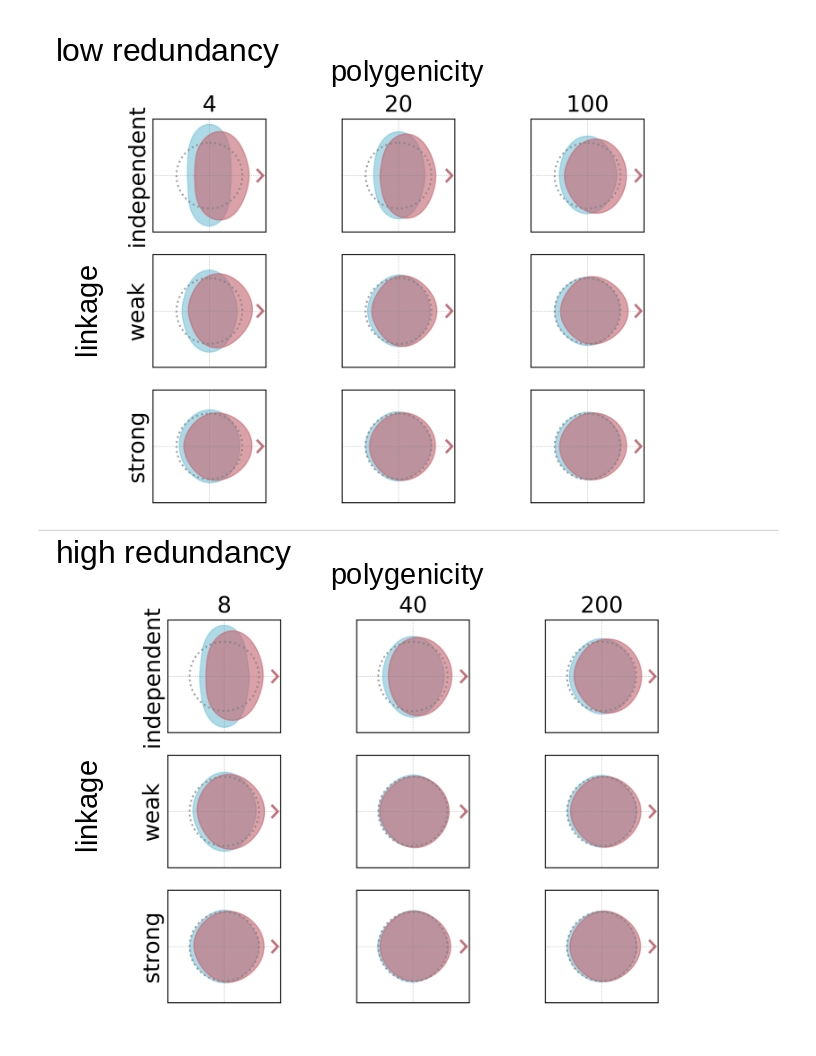
\includegraphics[width=.8\linewidth]{gene_flow_plots.jpg}
\caption{Comparison, across all 18 scenarios, of the distributions of gene-flow directions during the climate change period. Scenarios are organized as in Table 1, with rows for level of linkage and columns for number of loci per trait. Main scenarios (red) are compared against null scenarios (blue). Compass labels indicate directions of gene flow as it would be observed from a bird’s-eye view of the simulated landscape, with eastward gene flow moving in the same direction as the shifting environmental gradient (i.e., ‘upslope’), and with northward and southward gene flow being perpendicular to the environmental gradients (i.e., ‘on contour’). Westward gene flow would go against the direction of the shifting environmental gradient, and thus would be maladaptive under all scenarios, which explains why it is universally suppressed relative to the null results. There is a general trend toward increasing on-contour gene flow and decreasing upslope gene flow with increasing strength of linkage and increasing number of loci per trait..
}
\label{fig:gene_flow}
\end{figure*}

\subsection{Hypothesis 2: Linkage and polygenicity}
Our second hypothesis also met with partial support.
Mean fitness declined during climate change, at least temporarily, across all main scenarios, (GIVE ANOVA 
RESULTS; see Figure \ref{fig:fit_over_time_paneled}, as did population size (GIVE ANOVA 
RESULTS; see Figure S1).
Because of this, all scenarios displayed some maladaptation, as evidenced by the non-zero areas of the red wedges
in the 'after' scatterplots of Figures \ref{fig:pheno_shift} (low redundancy) and S2 (high redundancy).
The strength of these fitness and population declines was 
positively correlated with the strength of linkage, as we expected (GIVE HSD RESULTS),
but displayed a complex, non-linear relationship with polygenicity,
being steepest in high-polygenicity
scenarios (HSD RESULTS), less steep at low polygenicity, and minimal at
mid-polygenicity. 

\begin{figure*}[\sidecaptionrelwidth][t]
\centering
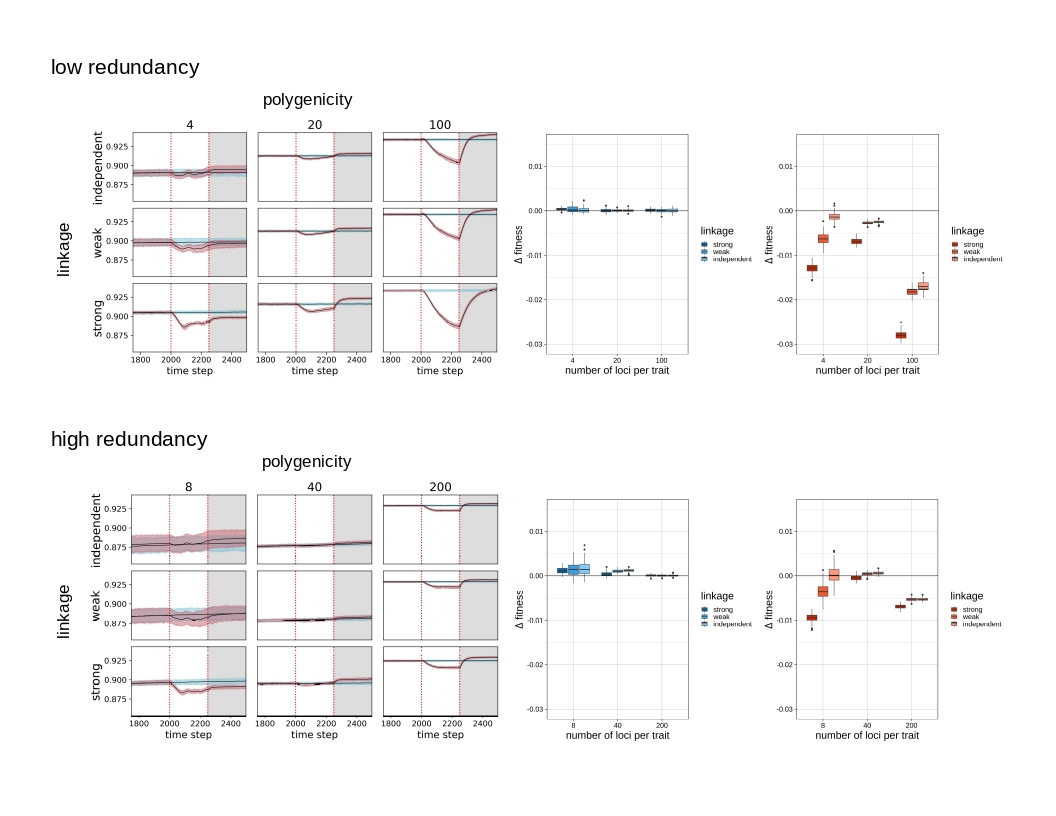
\includegraphics[width=17.8cm]{fit_time_series_and_boxplots.jpg}
\caption{Left: Mean fitness dynamics for all scenarios during the 250 time steps before the climate change period and the 250 time steps during it (with the two periods divided by a red, dashed vertical line marking the onset of the climate change period). Scenarios are organized as in Table 1, with rows for level of linkage and columns for number of loci per trait. Both means (black lines) and variability envelopes (5th percentile to 95th percentile) are shown, with scenario type depicted by color (main scenarios in red, null scenarios in blue). Right: Comparison of climate change-driven changes in mean fitness across scenarios. Null scenarios are plotted on the left in blue, and main scenarios are plotted on the right, in red. Within each plot, scenarios are divided by the number of loci per trait (x-axis) and by the strength of linkage (shade, with darker hues representing stronger linkage). Asterisks above each box indicate level of significance (*=0.1, **=0.05, ***=0.005).}
\label{fig:fit_over_time_and_boxplots}
\end{figure*}



\begin{figure*}
\centering
\includegraphics[width=17.8cm]{pheno_shift.jpg}
\caption{Comparison, across all 18 scenarios, of the observed versus expected phenotypic shift during the climate change period. Scenarios are organized as in Table 1, with rows for level of linkage and columns for number of loci per trait. For each scenario, the left scatterplot shows the distribution of individuals’ bivariate phenotypes before climate change begins (‘before’ columns), whereas the right scatterplot shows how the distribution has shifted by the end of the climate change period (‘after’ columns). The trait adapted to the shifting environmental gradient is distributed along the x axis, and the trait adapted to the stable gradient is distributed along the y axis. Scatterplots depict multi-model ensemble results for each scenario. The size and opacity of each point represents the number of individuals exhibiting that bivariate phenotype. (Note that the gridded arrangement of the points in each scatterplot is a function of the number of loci per trait which, because locus effect sizes are fixed, directly determines the set of attainable, evenly-spaced, discrete phenotypic values. Because fewer loci per trait yields fewer possible phenotypes, individuals are grouped into fewer, larger phenotypic bins in the 4- and 20-locus scenarios.) Solid black lines delineate the shift in the phenotypic distributions’ central tendencies that is expected to take place during the cimate change period, dotted black lines depict the observed (OLS-fitted) phenotypic distributions’ central tendencies at the ‘during’ and ‘after’ time steps, and translucent red wedges depict the differences between the expected and observed distributions (i.e., ‘phenotypic shortfall’, the response variable in our statistical tests).
}
\label{fig:pheno_shift}
\end{figure*}


Notably, declines were much stronger in the high-polygenicity, low-redundancy scenario
than in all others, with mean fitness
declining by XXXXXX\% on average (from XXX to XXX),
and mean population size declining by 19\% on average (from ~10,500 to ~8000 individuals).
Maladaptation was substantially higher in these scenarios too,
especially when linkage was strong. 
In fact, maladaptation was so strong that local extinction occurred
in the fastest-changing, rightmost extreme of the landscape,
as evidenced both by the scarcity of points in the bottom-central regions
of the post-change scatter plots (rightmost column, Figure \ref{fig:pheno_shift})
and the near-zero post-change population densities in the rightmost region of the landscape
(rightmost column, Figure S3; cf. Figure S4).
Crucially, declines were uniquely persistent in all high-polygenicity scenarios,
with no evidence of evolutionary rescue during climate change --- i.e., stabilization and rebound only occurred during the post-climate-change period,  showing that climate change outstripped adaptive capacity in these scenarios.
Conversely, the 4- and 20-locus scenarios showed varying degrees
of decline (HSD RESULTS) but all featured at least partial evolutionary rescue by the end of the climate change period.
 DISCUSS THE 'BUMPINESS' OF THE 4-LOCUS SCENARIOS?? 





\subsection{Hypothesis 3: Redundancy}

Our third hypothesis was fully corroborated by our results.
Across scenarios, high redundancy facilitated adaptation to environmental,
leading to less-pronounced declines in mean fitness and population size
(Figure \ref{fig:fit_over_time_paneled} and Figure S1, bottom)
and less maladaptation (Figure \ref{pheno_shift}, bottom).
This is not to say that adaptation successfully occurred in all circumstances,
though: fitness and population declines were still persistent in high-polygenicity scenarios.



\section*{Discussion}

Our analysis provides important theoretical insights
into the nature of polygenic adaptation under multivariate environmental change,
a neglected area of research.
While we confirm that some principles derived from previous models of local adaptation to static environments
also apply to changing environments, we simultaneously
reveal dynamics that would not be evident on that basis.
Our results generally support the first-order assumption underlying AGF,
but also suggest that if theoretical landscape genetics can cast 
light on the processes underlying maladaptation, adaptive capacity, and adaptive gene
flow, it can help answer the fundamental question posed by AGF: Whom to move where?

-------------------------

1-2 PARAGRAPHS HERE DISCUSSING RESULTS PRESENTED ABOVE, IN ORDER OF HYPOTHESES

DISCUSSION OF MAIN CONTRADICTIONS/UNEXPECTED RESULTS (BELOW, BUT CONDENSED)

SINGLE PARAGRAPH ABOUT FUTURE DIRECTIONS

SHORT CONCLUSION PARAGRAPH (Our study provideds insights into polygenic adaptation to environmental change, a neglected area of research. It confirms some principles derived from previous models of local adaptation to static environments, but also suggests that environmental change complicates the story in nuanced ways that are poorly covered by current theory. Much work remains to be done to better elucidate this area of research, and our work points at next steps.)

------------------------

Despite the general agreement between our hypotheses and our results,
our findings appear to complicate or contravene theoretical expectations in three major ways.
First, the dramatic degree of population decline observed in the low-redundancy, high-polygenicity
scenarios was unexpected,
as was the weak adaptive capacity in all of these scenarios, irrespective of 
linkage (right columns of Figures \ref{fig:fit_over_time_paneled} and S1).
Previous work has found that genetic architectures composed
of many genes of small effect produce stable, resilient phenotypic clines despite transient genotypic composition \cite{yeaman_amnat,yeaman_review},
leading to the expectation that species with highly polygenic climate-adaptative architectures 
may experience rapid local adaptation \cite{aitken_yeaman}. 
Despite that, we expected evolutionary responses to climate change
to be slower in these architectures
because natural selection is less effective on smaller-effect alleles
and because high linkage leads to longer expected wait times to generation
of novel, adaptive recombinants.
Nonetheless, we did not expect these scenarios to show a complete failure to adapt.

Given the polygenic nature of many complex ecological traits \cite{barghi_polygenic,boyle,rockman,savolainen,sella},
it is plausible that our high-polygenicity scenarios are realistic.
The dramatic results of the high-polygenicity, low-redundancy simulations,
which disappear in the high-redundancy scenarios,
thus position redundancy as a key determinant
of adaptive outcomes under climate change.
This raises important questions for further research:
1.) Is the low redundancy modeled here realistic, and if so, in which systems and settings?
2.) Are our findings robust to variation in other parameters
not explored here (e.g., effective population size, migration rate, rate of climate change)? 
It is possible that our high-polygenicity, low-redundancy scenarios
(and particularly, the rightmost edge of the landscape in those scenarios)
provide a good model of populations
at the warm edge of a species' range, where climate-adapted phenotypes have already
reached an extreme and where further adaptation is not likely
on the basis of standing diversity alone --- in other words, that warm-edge
populations have intrinsically low segregating redundancy,
which is likely to play a bigger role than genotypic redundancy and \textit{de novo} mutation
in adaptation to rapid environmental change \cite{laruson}.
Thus, efforts to identify predictors of segregating redundancy in the wild,
and efforts to identify other covariates of maladaptation in such populations,
could help identify species that are intrinsically evolutionarily vulnerable to climate change
(as has been proposed for forest trees \cite{lind,aitken_yeaman})
and help delineate the most vulnerable populations within them
(lending greater theoretical depth to recent mapping efforts \cite{bay,gougherty}).

A second complication relates to recombination,
which theory suggests can be deleterious
in situations of clinal adaptation
with gene flow, because recombination disrupts the association between adaptive loci 
underlying a single trait \cite{tigano}.
Our results highlight an interesting and important caveat here.
While the above expectation applies in the special case of a single-trait 
adapted to a single gradient,
it may change under other realizations of the 
generalized $n$ trait adapted to $\leq n$ gradients.
In our two-trait, two-gradient model, given that the gradients decouple
and novel environments emerge,
recombination is advantageous.
This is because, despite the fact that recombination disrupts the association between
adaptive loci for the shifting gradient's trait, preventing the
generation of larger-effect gene clusters,
it simultaneously dissociates those loci from the loci underlying
the stable gradient's trait, for which gene flow would be maladaptive.
In other words, recombination facilitates adaptation by gene flow
by providing escape from the genetic conflict that arises
from two separate and complex genetic architectures.
   
Third, given that our mid-range 20-locus scenarios
showed the least fitness and demographic impact of climate change,
and the quickest ability to adapt,
our results seem to contradict previous findings that adaptation on a cline tends to 
occur either by few genes of large effect or by many genes of small effect 
\cite{yeaman_amnat,yeaman_review}. 
This apparent contradiction may be partly explained by a 
difference in timeframes between adaptation to a static environmental gradient
and adaptation to a gradient undergoing environmental change. 
Adaptation to a single, static gradient can proceed gradually,
and may favor large-effect alleles or allele-clusters,
once they arise by mutation, recombination, gene flow, or some combination thereof. 
To the contrary, the sudden onset of persistent environmental change 
in a population that is already locally adapted initiates a 'race against time', 
and it may be that the genetic architectures with
optimal adaptive capacity are those that comprise freely recombining loci with small-enough effect sizes to avoid large
sudden declines in fitness from migration load,
but with large enough effect sizes to avoid the long wait times necessary for recombination to cluster many adaptive loci into larger-effect haplotypes.
In theoretical models, local adaptation with migration along static 
gradients tends to favor concentrated genetic architectures ---
those featuring linked allelic clusters with concomitantly larger effect sizes.
However, there is some evidence that in temporally fluctuating environments the opposite may be true:
adaptation may favor dispersed genetic architectures with higher rates of recombination
\cite{burger,kondrashov,yeaman_review,yeaman_whitlock}.
This suggests an inherent tension between the architectures that
might be expected to evolve in locally adapted populations prior to climate change
and the architectures most likely to facilitate adaptation to change --- though it remains to be determined how 
often and when concentrated genetic architectures actually occur in 
real-world systems \cite{laruson}).
It also suggests a mechanism by which species living in climates with 
less interannual fluctuation and longer-term stationarity could have
higher intrinsic vulnerability to maladaptation under climate 
change. Further research, both empirical and theoretical,
can help determine if such phenomena occur, and if so,
if they can inform and help prioritize efforts to enhance species'
adaptive capacity to climate change.



Indeed, managers seeking to enhance species' climate resilience
are increasingly relying on that assumption
through a practice known as `assisted gene flow` (AGF) \cite{aitken_whitlock},
in which individuals are brought into a focal population
from 'climate-suitable' populations \cite{bellis}.

Despite those complications, our results lend strong, generalized support to the foundational logic of AGF.
Up-gradient gene flow increased under climate change in all scenarios compared to the null,
indicating that even if it is maladaptive it is less so than only \textit{in situ} evolution.
However, our results also suggest that AGF is much less effective when traits
are underlain by many genes that are more tightly linked.
This is likely to be a more realistic portion of parameter space,
given the high expected polygenicity
of many complex, ecologically-relevant traits. However, some empirical work
details highly-polygenic traits with widely distributed effect sizes, in which case the small
subset of loci in the right tail of the effect-size distribution could in effect
behave like the low-polygencity, large-effect-size scenarios we present here.
Further research, both empirical and theoretical, will help clarify the
applicability of our various scenarios to real-world systems.
 
The major challenge in simulation-based research is the complexity of the high-dimensional 
parameter space that can be explored. Informative studies can be constructed by focusing on a 
small set of key parameters and exploring their influence
on the outcomes of interest, while holding other parameters at reasonable values. We have 
attempted to do that here. Nonetheless, some of the parameters we held constant here are certain 
to have important effects on our outcome of interest.
Exploration of those parameters would provide a more comprehensive,
mechanistic understanding of the nature of adaptation to environmental change. The foremost of these, 
which are areas ripe for future research, are:
    \begin{enumerate}
        \item \textit{population size}, a key determinant of the relative strengths of drift and natural selection \cite{murray} and of the wait time to emergence of recombinant haploytpes \cite{christiansen}, among other important dynamics;
        \item \textit{migration} (as either a fixed distance or a distribution \cite{paulose}), a key factor embedded in the rudimentary migration-selection dynamics that lie at the heart of models like ours \cite{wright,haldane,barton}, and the fundamental process motivating the practice of AGF;
        \item \textit{distributed allelic effect sizes} \cite{orr}, including whether clustered genetic architectures tend to emerge as a basis of local adaptation \cite{yeaman_whitlock} and, if so, what influence that has on the nature and likelihood of adaptation under rapid environmental change;
        \item variability in the slopes of environmental gradients, the rates of environmental change, and the spatial heterogeneity of those rates.
    \end{enumerate}
A variety of other facets of spatiotemporal evolution could also be explored 
through a similar modeling framework, including and genomic positions; 
pleiotropy \cite{thompson} and epistasis; more complex spatial 
arrangements \cite{benes};
variation in life history (e.g., number of offspring; discrete versus overlapping generations);
and mutation (although the relevance of \textit{de 
novo} mutation to climate change adaptation in the often long-lived 
and long-generation-time species of conservation concern is questionable
and deserves further work).
Finally, important and conservation-relevant insight could emerge from the 
integration of other dimensions climate change ecology, including range shifts 
\cite{weiss-lehman}, plasticity \cite{chevin} and heritable epigenetic variation,
and range-wide variation in population density \cite{aitken_whitlock}.


\matmethods{

\subsection*{Simulation}

We built all of the simulations for this study using \texttt{geonomics} \cite{terasaki_hart},
a Python \cite{rossum} package for
creating forward-time, agent-based, continuous-space landscape genomic simulations 
using arbitrarily complex life histories, environments, and environmental change 
scenarios. We created a base scenario for our set of simulations
by creating a \texttt{geonomics} template
parameters file featuring a species with two traits, each of which experiences 
selection on the basis of a different environmental variable (using the \texttt{geonomics.make\_parameters\_file} command).
Both environmental variables are modeled as linear, horizontal gradients
that span environmental values from 1 to 0, west to east.
During the simulation, one of these layers undergoes an environmental change 
event in which the gradient’s values change stepwise over a period of 250 time steps,
resulting in a final gradient that spans values from 1 to 0.5, west to east.
This creates a scenario in 
which two environmental variables become decoupled, leading 
to the emergence of novel environments (i.e. sites occupying new vectors in 
two-dimensional environmental space). Our goal here was to emulate a common 
phenomenon under climate change: the decouplin of multivariate environmental gradients,
leading to the emergence of novel climates \cite{williams_novel_climates,williams_projected_novel_disappearing,fitzpatrick_climate_novelty_forecasts}.

Individuals' phenotypes are determined by the additive effects of multiple loci (i.e., without pleiotropy or epistasis) --- a reasonable approximation of many traits of interest in real populations \cite{sella}.


Importantly, this landscape arrangement also generate heterogeneous rates of climate change,
with the rate ranging from 0 at the western edge to $0.5/250 time steps$ at the eastern edge.
This complicates interpretation of our results,
but much less so than in an alternative scenario
with spatially homogeneous rates of change,
which would have experienced range expansion as well as adaptation
during the climate change period.
The latter approach is also of interest,
and will be explored in future work,
but the approach we chose here allowed us
to best isolate evolutionary dynamics
resulting from the components of genetic architecture
that define our scenarios and hypotheses.

We then wrote a custom script in Python that reads that template \texttt{geonomics}
parameters file, 2.) edits any parameters that vary 
across our scenarios, 3.) instantiates a model, 4.) runs a fixed number of iterations 
of that model, and 5.) outputs custom data of interest. The parameters of interest, 
and the values they were assigned, are: the number of loci underlying each trait 
(parameter \texttt{n\_loci}: low = 5, moderate = 20, high = 100), the linkage between 
neighboring loci (i.e., the homogeneous recombination rate parameter, parameter \texttt{r}: unlinked = 
0.5, weak linkage = 0.05, strong linkage = 0.005), and the amount of genetic redundancy
(the \texttt{n\_loci} values specified above produce many-to-one genotype-phenotype mappings
at intermediate phenotypes that decline to become one-to-one mappings at extreme phenotypes,
whereas a doubling of those values produces many-to-one mappings across
all phenotypes that match available environmental values (i.e., phenotypes between 0 and 1, inclusive); see Figure S3 ).

(We did not include neutral loci in our simulations because genetic
hitchhiking would preclude them providing unique information
in all but the unliked scenarios. We also model strictly additive locus effects,
with no pleiotropy or epistasis.)
The full factorial combinations
of the chosen values of those parameters generate the set
of simulation scenarios laid out in
the central grid of Table 1. We used that script to run a set of batch jobs on the 
savio3 partition of UC Berkeley’s Savio system (each node has 96 GB RAM and 32, 
2.1-GHz Skylake processors). For each scenario, we ran a total of 100 iterations of 
the scenario of interest, featuring a 250-time-step climate change period (henceforth, 
the ‘main’ scenarios), and 100 iterations of a paired null scenario without natural 
selection (henceforth, the ‘null’ scenarios). 


Given that \texttt{geonomics} is a complex simulation framework, it features numerous other 
parameters whose values could be set or explored by the user. For the vast majority of
these parameters we left them set at reasonable default values. However, the 
parameters that we deemed as having high potential influence over results despite not 
being of particular interest for our study (henceforth, ‘nuisance parameters’) were 
set to low, high, and middle values within a reasonable range. NUISANCE PARAMETERS 
INCLUDED… This generated independent datasets for each value of each nuisance 
parameter. We reran our main analyses, as explained below, for each of these 
independent datasets, allowing us to characterize sensitivity of our results to each 
nuisance parameter. (For the complete set of \texttt{geonomics} parameters, and the values 
assigned to them across all models, see Appendix XXX.) ORGANIZE THIS APPENDIX AS A GNX
PARAMETERS FILE WITH MULTIPLE VALUES DISPLAYED AND HIGHLIGHTED IN GREEN FOR KEY PARAMS
OF INTEREST AND MULTIPLE VALUES DISPLAYED AND HIGHLIGHTED IN ORANGE FOR NUISANCE PARAMS.


Using a combination of internal \texttt{geonomics} functions and custom Python code, we 
designed a set of data outputs from each model run that would allow us to test our 
series of hypotheses. We saved tables of individuals’ locations and phenotypes at both
the beginning and the end of the climate change period. We also saved time 
series of population size, mean fitness, and mean phenotype of the trait adapted to 
the shifting gradient. We gathered this data at every time step, from 250 time steps 
before the onert of climate change, through the 250 time steps of the event, and 
continuing until 250 time steps after climate change completed.
The final 250 time steps after climate change were unrealistic, but nonethless helped elucidate
the nature of the changes that persisted at the end of the climate change period;
we thus refer to this period as the 'post-change diagnostic period'.
Lastly, we saved data on the vector directions of all gene flow during the 
climate change period, extracted from the spatial pedigrees stored in the
\texttt{tskit} \cite{kelleher} 
data structures. From that full set of gene flow data we calculated a pair of measures
of gene flow directionality,  which we refer to as ‘eastness’ (i.e., up-gradient 
directionality) and ‘north-southness’ (i.e., on-contour directionality). These were 
calculated as:

$Eness = \frac{\sum\limits_{i}^{n}\cos\theta}{n},\ \cos\theta\geq0$,

$NSness = \frac{\sum\limits_{i}^{n}|\sin\theta|}{n}$,

where angles are expressed counterclockwise from east. We ignored westness because 
gene flow in that direction is expected to be low irrespective 
of scenario, given that it would oppose the environmental shift and would almost 
always be maladaptive. We also saved a subsample of the full set of gene flow 
direction data by keeping all data pertaining to two randomly chosen loci that had 
positive effects on the trait adapted to the shifting environmental gradient. We 
restricted our sample in this way both to focus on loci expected to facilitate 
adaptation to increasing environmental values and thus to shift upslope, and to 
provide equal sample sizes across scenarios in downstream analysis (which was 
constrained to the number of positive-effect loci present in the four-locus-per-trait 
scenarios, i.e. two). 


For each of our 18 scenarios, and for both main and null scenarios, we ran 100 
iterations and generated 100 of the output data sets described above. We then 
generated visual summaries and ran statistical analyses across all simulations’ 
datasets. All analysis and visualization was produced using custom scripts written in 
Python and R \cite{r_core_team}.

\subsection*{Analysis}

To probe our hypotheses about climate change-driven shifts in population size, 
mean fitness, and mean phenotype of the shifting-gradient trait, we first plotted the 
trajectories of these metrics in each of our 18 scenarios. For each scenario, and 
for both main and null models, we created ensemble datasets by combining all 100 
iterations’ population size and mean fitness time series outputs. For each time step 
in the time series we calculated the mean and the 5th and 95th percentiles. Then we 
plotted, across all scenarios, the resulting trajectories of the means and their 
variability envelopes, for population size (Figure 1), mean fitness (Figure 2), and 
mean phenotype of the shifting-gradient trait (Figure S1). We plotted these metrics 
from 250 time steps before the climate change event until 250 time steps after 
its completion, allowing us to visualize the onset, course, and aftermath of the 
change event. 


To test our hypotheses about population size and mean fitness, we calculated a single 
metric of change over the course of the climate change event (, where x can be 
either population size or mean fitness) for each run of each scenario. We then ran a 
two-way ANOVA of each one, partitioning variance as a function of the two independent 
variables that defined our scenarios (number of loci per trait; strength of linkage). 
We ran \textit{post hoc} Tukey’s honest significant difference (HSD) tests each time an ANOVA 
showed overall significant results, to determine which levels of our independent 
variables showed divergent results. Lastly, we repeated this analysis for all null 
simulations, as a control.


To test our hypotheses about the pace of phenotypic shift across scenarios, we 
developed a metric of ‘persistent maladaptation shortfall’, then compared it across our grid of 
scenarios. We defined ‘persistent adaptation’ as the difference between: a.) the area 
within two-dimensional trait space that the population’s phenotypic distribution 
should have shifted across during the climate change event so as to remain 
optimally fit to its environment, and b.) the observed area of phenotypic shift within
a simulation. (We refer to this metric as 'persistent' to emphasize that it does
not reflect intermittent maladaptation that arises but then resides during the period of climate
change, but instead reflects maladaptation that remains at the end of the
climate change period.) To measure this area, we first determined the triangular area between 
the expected central tendency line of the optimal bivariate phenotypic distribution 
before the climate change event and the same line of optimal distribution after 
the event. The expected central tendency lines that delineate this area are clearly 
set by the model parameterization: they are the lines connecting all of the discrete 
points in environmental space that occur on the pre- and post-change landscapes. For 
each model run, we used ordinary least squares (OLS) to fit a best-fit trend line to 
the observed phenotypic distribution of the population at the end of the environmental
change event (arithmetically fixing the y-intercept at the (1,1) point in phenotypic 
space, which is the unchanging phenotypic optimum at the righthand extent of the 
landscape). We then calculated the phenotypic shortfall as the area of the wedge 
between the expected and observed post-change central tendency lines of the 
population’s phenotypic distribution. We calculated phenotypic shortfall for each 
model run, then used two-way ANOVA to test for a difference of means as a function of 
number of loci per trait and strength of linkage. Additionally, we used post-hoc HSD 
tests to further explore the observed differences in phenotypic shift across our 
scenarios. Finally, we used the ensemble data from all model runs to visualize this 
analysis in Figure XXX, including the observed phenotypic distributions before, 
during, and after climate change (scatterplots), expected distributional central
tendencies before and after change (solid lines), observed central tendencies (dotted 
lines), and observed phenotypic shortfalls (translucent red wedges).

To visually investigate our hypothesis about the predominant directionality of gene 
flow under each scenario, we first produced a visualization of the directional 
distributions of gene flow in all 9 scenarios, compared between main and null 
scenarios (Figure 7). From each model run we gathered directional data for a random 
sample of the gene flow that occurred during the climate change event, using 
\texttt{geonomics} integration with \texttt{tskit} \cite{kelleher}, which allows for temporal 
subsetting and output of the information contained the full spatial pedigree of a 
population. We then fitted a mixture of 4 von Mises distributions to that data, 
yielding 12 parameter estimates defining the fitted mixture distribution. For each of 
the 18 scenarios, we then plotted the mean of the probability density functions 
described by each of those length-12 vectors of fitted parameters. We did this 
separately for null scenarios and for main scenarios, then overlaid the null and main 
results, providing a summary depiction of the nature of gene flow within each 
scenario, compared to its null expectation.

To test our hypotheses about the direction of gene flow, we ran two-way ANOVAs of 
eastness and north-southness (with Bonferroni correction for multiple testing), 
followed by post hoc HSD tests. We also ran this analysis for null simulations, as a 
control.

} % end matmethods


\showmatmethods{} % Display the Materials and Methods section

\acknow{We thank A. Bishop, T. Dawson,  J. Frederick, N. Graham, M. Kelly, M. McElroy, E. Westeen, G. Wogan, and M. Yuan for feedback and guidance on various iterations of the simulations presented herein. We thank Berkeley Research Computing for providing access to the Savio computing cluster. We thank D. Ehrenfeld, N. Fefferman, M. Fitzpatrick, and L. Plough for cultivating an interest in conservation genetics. Lastly, we thank M. Terasaki Hart, C. Nemec-Hart, G. Hart, J. Hart, and M. Tylka for supporting and encouraging a lifetime of curiosity about nature, and C. S. aTunde Adjuah, B. Evans, R. Pérez Joglar, Y. Y. Ma, and J. Redman for the pleasant solitude. This work was supported by a Berkeley Fellowship (to D.E.T.H.) and by National Science Foundation grant DEB1845682 (to I.J.W.).}

\showacknow{} % Display the acknowledgments section

% Bibliography
\bibliography{terasaki_hart_ch2}

%%%%%%%%%%%%%%%%%%%%%%%%%%%%%%%%%%%%%%%
% TEMPORARY PLACE FOR SUPPLEMENTAL FIGS

\textbf{SUPPLEMENTAL FIGS:}


\begin{figure*}[\sidecaptionrelwidth][t]
\centering
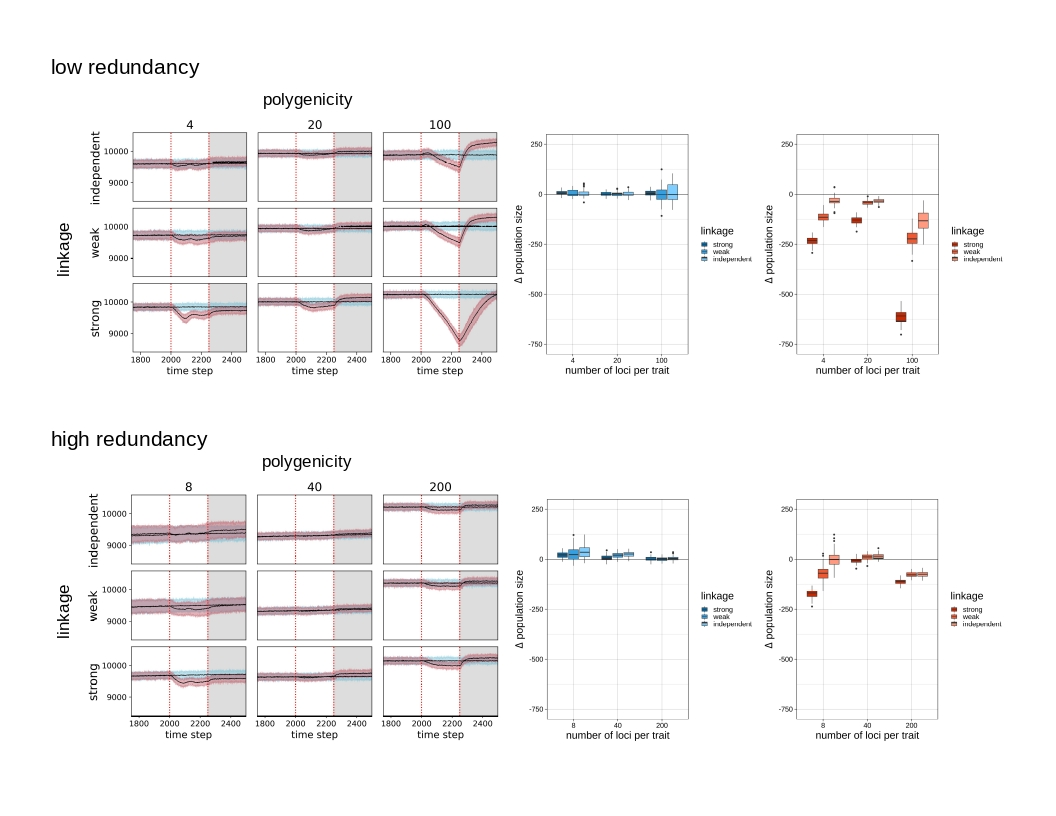
\includegraphics[width=17.8cm]{Nt_time_series_and_boxplots.jpg}
\caption{Left: Population size dynamics for all scenarios during the 250 time steps before the climate change period and the 250 time steps during it (with the two periods divided by a red, dashed vertical line marking the onset of the climate change period). Scenarios are organized as in Table 1, with rows for level of linkage and columns for number of loci per trait. Both means (black lines) and variability envelopes (5th percentile to 95th percentile) are shown, with scenario type depicted by color (main scenarios in red, null scenarios in blue). Right: Comparison of climate change-driven changes in mean population size across scenarios. Null scenarios are plotted on the left in blue, and main scenarios are plotted on the right, in red. Within each plot, scenarios are divided by the number of loci per trait (x-axis) and by the strength of linkage (shade, with darker hues representing stronger linkage). Asterisks above each box indicate level of significance (*=0.1, **=0.05, ***=0.005).}
\label{fig:S1}
\end{figure*}


\begin{figure*}
\centering
\includegraphics[width=.8\linewidth]{pub/density_shift.jpg}
\caption{Maps depicting shifts in population density during climate change for all scenarios.}
\label{fig:S2}
\end{figure*}


\begin{figure}
\centering
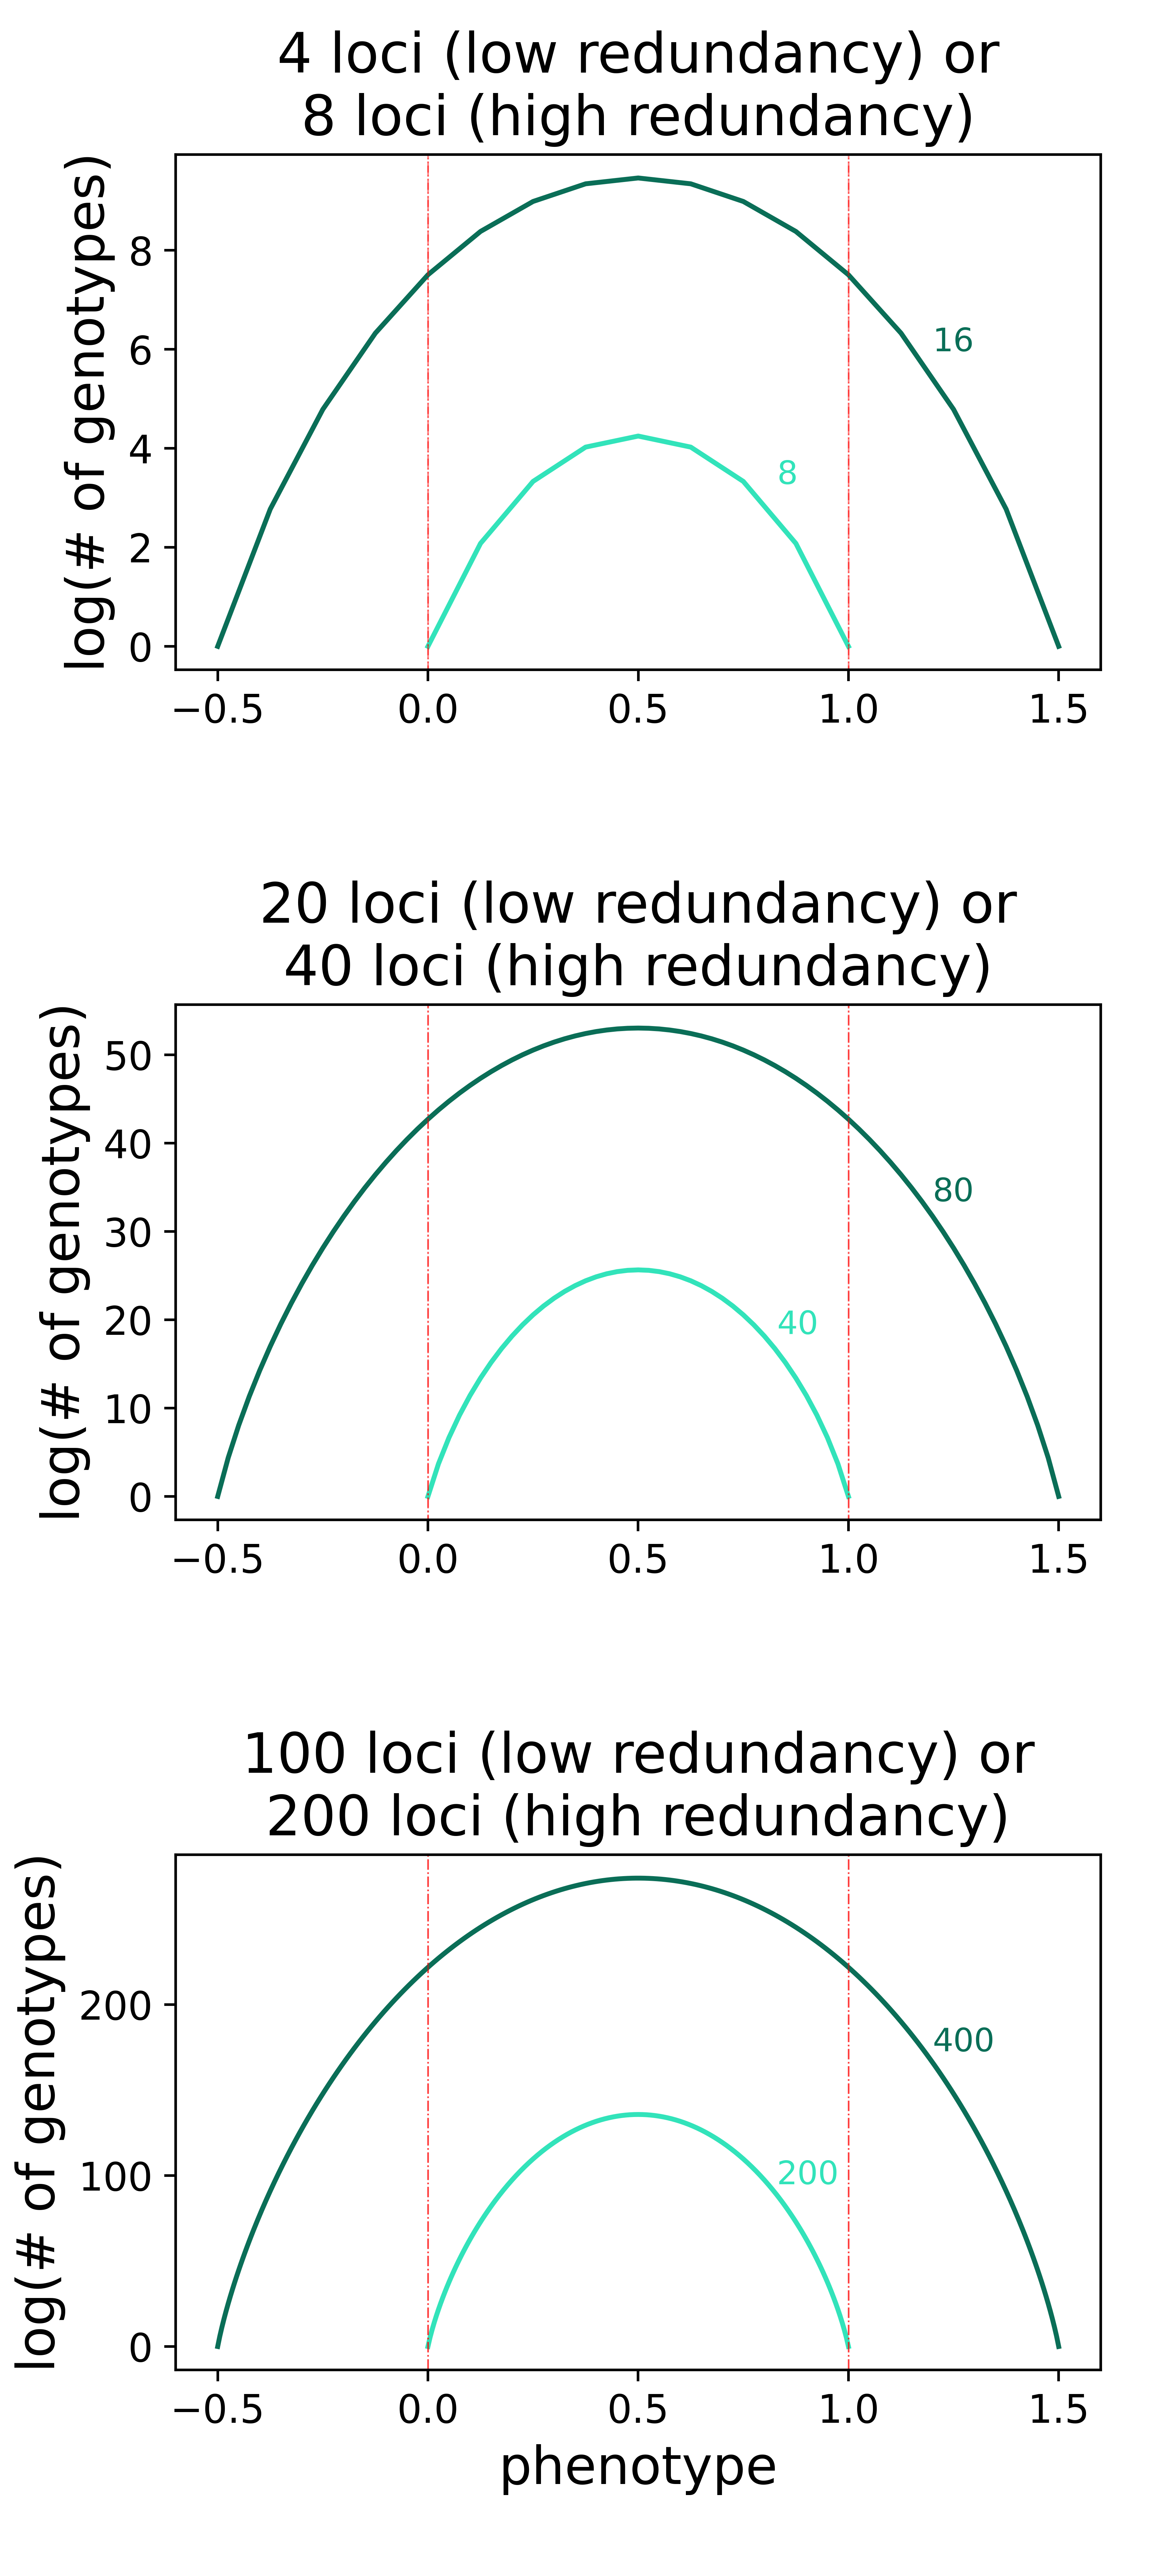
\includegraphics[width=.8\linewidth]{redundancy_fig.png}
\caption{Depiction of redundancy for all simulated polygenicity values. Phenotypic values are plotted along the x-axis, and the natural log of the number of genotypes that yield each phenotypic value is plotted along the y-axis. Polygenicities corresponding to low-redundancy scenarios are plotted and labeled in light teal, and those corresponding to high-redundancy scenarios in dark teal. The minimum and maximum environmental values on the landscape are represented by dotted vertical lines. The number of genotypes corresponding to each phenotype is calculated using a custom adaptation of Eqxn. ii, Box 1 in \cite{laruson}, implemented for a diploid species and fitted to the numerical conventions used by Geonomics.
}
\label{fig:S3}
\end{figure}

%%%%%%%%%%%%%%%%%%%%%%%%%%%%%%%%%%%%%%%

\end{document}
